\begin{ledgroupsized}[r]{120mm}%
\footnotesize%
\pstart%
\noindent\textbf{\"{U}berlieferung:}%
\pend%
\end{ledgroupsized}%
\begin{ledgroupsized}[r]{114mm}%
\footnotesize%
\pstart%
\parindent -6mm%
\makebox[6mm][l]{\textit{L}}%
Aufzeichnung: LH XXXV 12, 2 Bl. 150.
1 Bl. 2\textsuperscript{o}. Etwa \nicefrac{1}{3} S. auf Bl. 150~r\textsuperscript{o} mittig.
Das obere Drittel von Bl. 150~r\textsuperscript{o} überliefert das Stück \textit{LSB} VII, 3 N. 73.
Das untere Drittel ist leer.
Bl. 150~v\textsuperscript{o} überliefert einen algebraischen Text (Cc~2, Nr.~1515 B), der nachträglich in einem Band von \textit{LSB} VII gedruckt werden soll.
Ein Wasserzeichen.
\newline%
Cc 2, Nr. 1516%
\pend%
\end{ledgroupsized}%
%
% \normalsize
\vspace*{5mm}%
\begin{ledgroup}%
\footnotesize%
\pstart%
\noindent%
\footnotesize{%
\textbf{Datierungsgr\"{u}nde:}
Das Wasserzeichen im Textträger des vorliegenden Stücks N.~99 %?? = vorliegendem Stück = 35,12,02_150 
ist eigentlich für die Früh\-lings\-monate des Jahres 1676 belegt.
Wie die Editoren von \cite{01129}\textit{LSB} VII, 3 N. 73 jedoch bemerken (S.~834), bezieht sich Leibniz in N.~99 %?? = vorliegendem Stück = 35,12,02_150 
auf \cite{01128}\textsc{J.B. Tavernier}, \textit{Les six voyages}, 2 Bde, Paris 1676.
Dieses Buch wurde, wie im Kolophon beider Bände angegeben, erst am 1. Oktober 1676 vom Drucker abgeliefert. % (\textit{achevé d'imprimer})
Einem Brief Leibniz' vom Dezember 1676 entnimmt man ferner,
dass er noch vor seiner Abreise aus Paris (4. Oktober 1676) auf Taverniers neuerschienenes Werk aufmerksam geworden war
(\cite{01130}\textit{LSB} I, 2 N. 209, S.~239).
Die Editoren von \cite{01129}\textit{LSB} VII, 3 N. 73 schlagen demgemäß vor (S. 834), das vorliegende Stück N.~99 %?? = dieses Stück hier = 35,12,02_150 
auf Oktober bis Dezember 1676 zu datieren.
Dieser Vorschlag wird hier übernommen.%
}%
\pend%
\end{ledgroup}%
%
\vspace*{8mm}%
\count\Bfootins=1500
\count\Cfootins=1500
\count\Afootins=1500
\pstart%
\normalsize%
\noindent%
% [150 r\textsuperscript{o}]
[150 r\textsuperscript{o}] \edtext{}{\lemma{}\Afootnote{\textit{Am Rand:}
\protect\index{Sachverzeichnis}{acier}Acier tremp\'{e} ne rouille pas.\vspace{-4mm}}}%
Dans la chemine\'{e}\protect\index{Sachverzeichnis}{chemine\'{e}} il seroit
\edtext{bon qu'il y eut}{\lemma{bon}\Bfootnote{\textit{(1)}\ que la fa \textit{(2)}\ qu'il y eut \textit{L}}}
des faces mobiles pour dresser la chaleur\protect\index{Sachverzeichnis}{chaleur}
tantost vers les pieds tantost vers le corps, jamais vers les yeux.
On voit en cela l'effect de l'angle de reflexion.\protect\index{Sachverzeichnis}{reflexion}
\pend%
\pstart%
\edtext{Mons. Tauerni\protect\index{Namensregister}{\textso{Tavernier}, Jean Baptiste 1605-1689}
dit qu'on manque de bois\protect\index{Sachverzeichnis}{bois}
dans les deserts\protect\index{Sachverzeichnis}{désert} d'Arabie,\protect\index{Ortsregister}{Arabien}
quoyqu'on ne manque pas quelques fois de gibier,\protect\index{Sachverzeichnis}{gibier}
mais, qu'on ne le peut pas cuire.%
}{\lemma{Mons. [...] cuire}\Cfootnote{\cite{01128}\textsc{J.B. Tavernier}, \textit{Les six voyages}, Paris 1676, Bd. I, S. 147-149.}}
Je croy qu'un miroir ardent\protect\index{Sachverzeichnis}{miroir ardent}
qui fut mobile bien viste, pour passer sur la viande\protect\index{Sachverzeichnis}{viande}
en differens endroits, seroit excellent.
\pend%
\pstart%
Il faut voir s'il est
\edtext{possible tirer de l'air\protect\index{Sachverzeichnis}{air}
}{\lemma{possible}\Bfootnote{\textit{(1)}\ de tirer \textit{(2)}\ tirer de l'air \textit{L}}}
une quantit\'{e} d'eau\protect\index{Sachverzeichnis}{eau}
raisonnable par la seule pression.\protect\index{Sachverzeichnis}{pression}
Ce seroit d'un excellent usage dans les deserts\protect\index{Sachverzeichnis}{désert} d'arabie\protect\index{Ortsregister}{Arabien}.
\pend%
\pstart%
Grand usage des choses qui sont en m\^{e}me temps fermes et souples.
Il \edtext{faudroit porter sur}{\lemma{faudroit}\Bfootnote{\textit{(1)}\ avoir de \textit{(2)}\ porter sur \textit{L}}}
soy de quoy faire toutes sortes des choses.
Pour cet effect, il faudroit des pieces de fer\protect\index{Sachverzeichnis}{fer}
\pend
\newpage
\pstart\noindent
qu'on puisse demonter et rejoindre en plusieurs
\edtext{[fa\c{c}ons]}{\lemma{fa\c{c}on}\Bfootnote{\textit{L \"{a}ndert Hrsg.}}}
avec des vis
\edtext{[d']}{\lemma{d'}\Bfootnote{\textit{erg. Hrsg.}}}%
acier,\protect\index{Sachverzeichnis}{acier} pour limer, couper, percer.
\edtext{Toiles\protect\index{Sachverzeichnis}{toile}}{\lemma{Toiles}\Bfootnote{\textit{erg. L}}}
cir\'{e}es pliantes.
Miroir ardent.\protect\index{Sachverzeichnis}{miroir ardent}
\protect\index{Sachverzeichnis}{verre}Verre malleable.
\protect\index{Sachverzeichnis}{fer}Fer blanc car on en fait beaucoup
\edtext{de choses}{\lemma{de choses}\Bfootnote{\textit{erg. L}}}
aisement.
\protect\index{Sachverzeichnis}{fusil}Fusil et
\edtext{meche.\protect\index{Sachverzeichnis}{mèche}
Colle\protect\index{Sachverzeichnis}{colle}%
}{\lemma{meche.}\Bfootnote{\textbar\ (papier). \textit{gestr.}\ \textbar\ Colle \textit{L}}}
excellente.
\protect\index{Sachverzeichnis}{plomb}Plomb propre \`{a} faire des modelles,
pendant qu'il est encor chaud.
\pend%
\pstart%
On pourroit faire un miroir ardent\protect\index{Sachverzeichnis}{miroir ardent} compos\'{e} de plusieurs plaques
\edtext{plattes}{\lemma{plattes}\Bfootnote{\textit{erg. L}}} qui ne laisseroit pas de faire un grand effect.
\pend%
\pstart%
Si non posset explicari reflexionis\protect\index{Sachverzeichnis}{reflexio} causa nisi per
\edtext{elaterium,\protect\index{Sachverzeichnis}{elaterium}
nullae essent atomi;\protect\index{Sachverzeichnis}{atomus}%
}{\lemma{elaterium,}\Bfootnote{\textit{(1)}\ elaterium \textit{(2)}\ nullae essent atomi; \textit{L}}}
at inde sequeretur absurdum,
ut alibi. Ergo dicendum foret nunquam atomum atomo\protect\index{Sachverzeichnis}{atomus} concurrere.
\pend%
\pstart%
Pluma\protect\index{Sachverzeichnis}{pluma}
\edtext{minus}{\lemma{minus}\Bfootnote{\textit{erg. L}}}
tertia parte celeritatis\protect\index{Sachverzeichnis}{celeritas} suae ordinariae,
in tubo\protect\index{Sachverzeichnis}{tubum}
\edtext{bipedali}{\lemma{}\Afootnote{\textit{Über} bipedali: \Denarius\vspace{-4mm}}}
vitreo, aere\protect\index{Sachverzeichnis}{aer} exhausto descendit, et sine gyrationibus
\edtext{experimento\protect\index{Sachverzeichnis}{experimentum} Boylii.\protect\index{Namensregister}{\textso{Boyle}, Robert 1627-1691}%
}{\lemma{experimento Boylii}\Cfootnote{\cite{01062}\textsc{R. Boyle}, \textit{Continuation}, Oxford 1669, S. 139-142.}}
\pend%
\pstart%
Lingua $\phi$iloso$\phi$ica\protect\index{Sachverzeichnis}{lingua philosophica}
polietur cum philosophia.\protect\index{Sachverzeichnis}{philosophia}
\pend%
\pstart%
\edtext{Ferrum\protect\index{Sachverzeichnis}{ferrum} calore\protect\index{Sachverzeichnis}{calor} fit flexile,}{\lemma{Ferrum}\Bfootnote{\textit{(1)}\ chalibs durum \textit{(2)}\ calore fit flexile, \textit{L}}}
at orichalcum\protect\index{Sachverzeichnis}{orichalcum} loton\protect\index{Sachverzeichnis}{loton}
% \edtext{}{\lemma{loton}\Cfootnote{Wohl seltene Schreibweise (\textsc{Fureti\`{e}re}, \textit{Dictionnaire universel}, DenHaag 1702, o.S., \textsc{F\'{e}raud}, \textit{Dictionaire critique}, Marseille 1787, S. 531.548.571; auch leton, \textsc{Nicot}, \textit{Thresor}, Paris 1606, S. 365.) des franz\"{o}sischen laiton f\"{u}r orichalcum.}}
dum calet fragile est instar vitri.\protect\index{Sachverzeichnis}{vitrum}
\pend%
\pstart%
Mercatoris\protect\index{Namensregister}{\textso{Mercator}, Nicolaus 1620-1687}
secret das wasser\protect\index{Sachverzeichnis}{Wasser} zu heben
ohne r\"{a}der\protect\index{Sachverzeichnis}{Rad} und bewegung
durch den blossen fall,\protect\index{Sachverzeichnis}{Fall}
gleichwie man schohn es eben so hoch als zuvor
\edtext{gebracht. Cursus $AB,$}{\lemma{gebracht.}\Bfootnote{%
\textit{(1)}\ Ita ille %
\textit{(2)}\ Cursus %
\textit{(a)}\ $BC.$ %
\textit{(b)}\ $AB,$ \textit{L}}}
lapsus $BC,$ assurgit aqua ad $DE \sqcap BC$ ordinarie modo jam noto, ipse sustulit adhuc altius, et multiplicat quantumvis.
Adde Mariotte\protect\index{Namensregister}{\textso{Mariotte}, Edme 1620?-1684}
et Papin.\protect\index{Namensregister}{\textso{Papin}, Denis 1647-1714}
\pend%
\vspace*{2.0em}
\pstart%
\centering
% \begin{wrapfigure}{l}{0.4\textwidth}                    
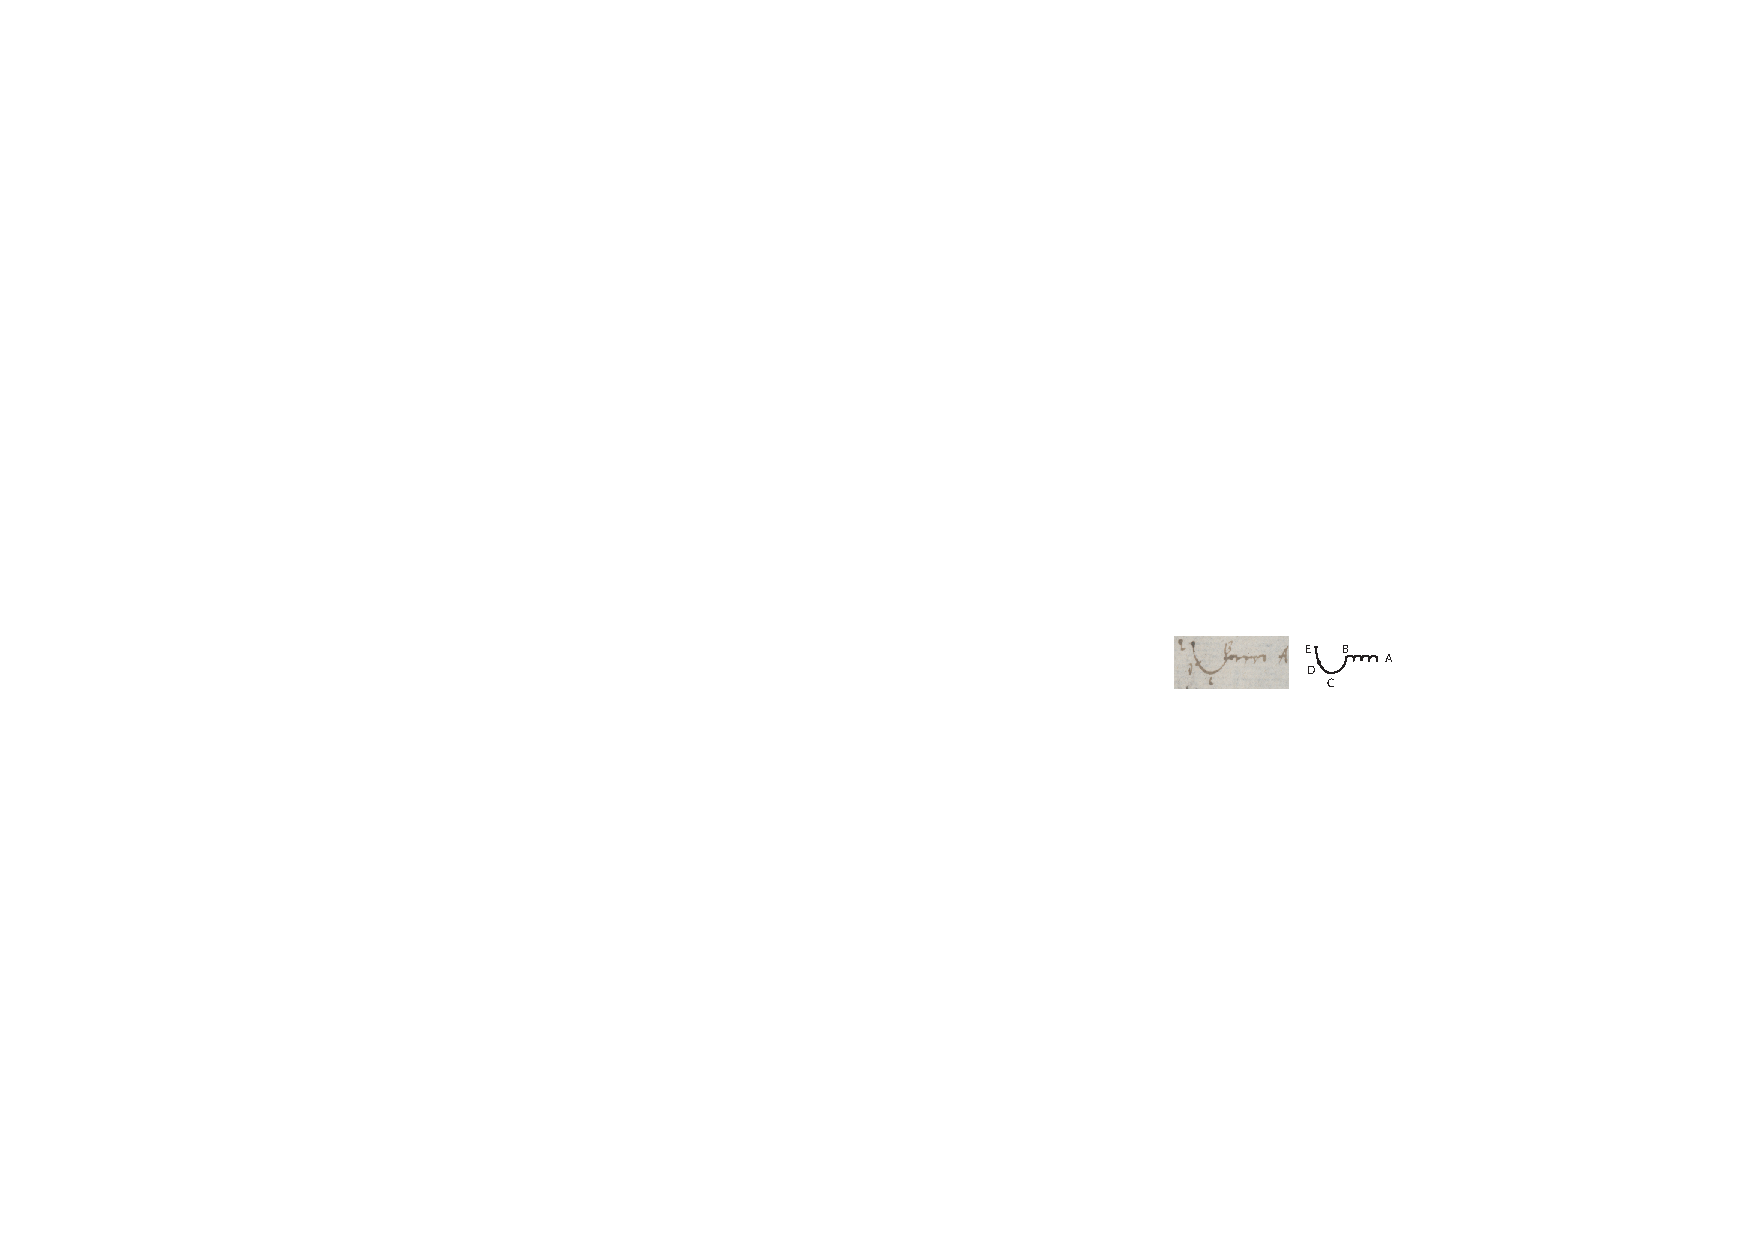
\includegraphics[width=0.55\textwidth]{images/lh0351202_150r-d1.pdf}\\
\centering
[\textit{Fig. 1}]
% \end{wrapfigure}
\pend%
\count\Bfootins=1500
\count\Cfootins=1500
\count\Afootins=1500